\documentclass[a4paper, english]{report}
\usepackage{babel}
\usepackage{csquotes}
\usepackage[utf8x]{inputenc}
\usepackage[T1]{fontenc}

\usepackage{multicol}

\usepackage{afterpage}
\usepackage{hyperref}
\usepackage{biblatex}
\usepackage[a4paper,top=3cm,bottom=2cm,left=3cm,right=3cm,marginparwidth=1.75cm]{geometry}
\addbibresource{bibliography.bib}

\usepackage{amsmath}
\usepackage{amsthm}
\newtheorem{definition}{Definition}
\newtheorem{notation}{Notation}

%%%%%%%%%%%%%%%%%%%%%%%%%%%%%%
% TIKZ stuff
\usepackage{tikz}
\usetikzlibrary{shapes, arrows, positioning,fit,calc, decorations, backgrounds}

\tikzset{
  -|-/.style={
    to path={
      (\tikztostart) -| ($(\tikztostart)!#1!(\tikztotarget)$) |- (\tikztotarget)
      \tikztonodes
    }
  },
  -|-/.default=0.5,
  |-|/.style={
    to path={
      (\tikztostart) |- ($(\tikztostart)!#1!(\tikztotarget)$) -| (\tikztotarget)
      \tikztonodes
    }
  },
  |-|/.default=0.5,
}

\newcommand{\asymcloud}[2][.1]{%
\begin{scope}[#2]
\pgftransformscale{#1}%    
\pgfpathmoveto{\pgfpoint{261 pt}{115 pt}} 
  \pgfpathcurveto{\pgfqpoint{70 pt}{107 pt}}
                 {\pgfqpoint{127 pt}{291 pt}}
                 {\pgfqpoint{200 pt}{273 pt}} 
  \pgfpathcurveto{\pgfqpoint{78 pt}{382 pt}}
                 {\pgfqpoint{381 pt}{445 pt}}
                 {\pgfqpoint{412 pt}{410 pt}}
  \pgfpathcurveto{\pgfqpoint{577 pt}{587 pt}}
                 {\pgfqpoint{698 pt}{488 pt}}
                 {\pgfqpoint{685 pt}{366 pt}}
  \pgfpathcurveto{\pgfqpoint{840 pt}{192 pt}}
                 {\pgfqpoint{610 pt}{157 pt}}
                 {\pgfqpoint{610 pt}{157 pt}}
  \pgfpathcurveto{\pgfqpoint{531 pt}{39 pt}}
                 {\pgfqpoint{298 pt}{51 pt}}
                 {\pgfqpoint{261 pt}{115 pt}}
\pgfusepath{fill,stroke}         
\end{scope}}    

\usepackage{rotating}
%%%%%%%%%%%%%%%%%%%%%%%%%%
\usepackage{xspace}
\newcommand{\tozti}{\textsc{Tozti}\xspace}

\title{
  \tozti Midterm Report ~\\[1cm]
  \large `Projet Intégré' --- \textsc{Ens} Lyon
}

% FIXME: use titlepage
\author{\begin{minipage}[c]{.8\textwidth}
\rule{\textwidth}{1pt}
\begin{multicols}{2}
\begin{itemize}
\item Léonard Assouline
\item Peio Borthelle
\item Guillaume Cluzel
\item Guillaume Duboc
\item Julien Ducrest
\item Lucas Escot
\item Joël Felderhoff
\item Félix Klingelhoffer
\item Romain Liautaud
\item Pierre Meyer
\end{itemize}
\columnbreak
\begin{itemize}
\item Alex Noiret
\item Pierre Oechsel
\item Lucas Perotin
\item Vincent Rebiscoul
\item Emmanuel Rodriguez
\item Daniel Szilagyi
\item Lucas Venturini
\end{itemize}
\end{multicols}
\rule{\textwidth}{1pt}
\end{minipage}}

\date{\today}

\begin{document}
\maketitle

\tableofcontents % at least temporarily, easier for outline

\newpage

\chapter{Introduction}
The ENS has a rich associative life, and many of the student associations require efficient means of internal organisation. Currently, they use software ranging from a simple email client to a fully custom solution for managing members, meetings and finances. The biggest player in the field of associative software is Adeline, developed by former ENS students who grew tired of manually managing their hundreds of members. Yet overall, the existing tools are well suited for public relations (e.g. informing members of upcoming events), but do not allow for efficient internal organisation (e.g. storing documents, meeting of the board, scheduling events, archiving the work that was done). Many student associations are therefore being dragged down, mainly due the tools they use, which are often unintuitive and do not integrate well with each other. Most notably, this leads to a lot of redundant \emph{plumbing} work, and makes it hard for users to locate the information they want, as it is scattered over multiple sources.

To solve those issues, the \tozti project will {\bfseries allow each association to build the unified organisation suite that best fits its needs} by choosing from a wide range of well-integrated modules. These modules, which we will develop over the course of the project, will each answer a specific organisational need: \emph{communicating} in a hierarchical manner, reaching \emph{consensus}, \emph{planning} tasks and events, \emph{archiving} files securely, \emph{collaborating} on textual documents, or even \emph{automating} recurring tasks.

We ultimately want to build a service that student associations can use straight away. To this end, we maintain close communication with their representatives, to ensure that what we are building suits their needs.

In an effort to be flexible, our software architecture will revolve around small, loosely-coupled but interoperable modules, which we will build using today's web standards and best practices.


% * Brief overview of the state of the art of associative software.
% * The problem we are solving.
% * Section overview.



\chapter{Specification}
\label{chap:Specification}
% What exactly do we want from our platform (user and developer usecases)
% * user expectations
%   * unified overview of associations (and other groups)
%     -> dashboard
%     -> tree-like view
%   * forum
%   * (media) file "cloud"
%   * calendar (+remainders, +permit)
% * dev expectations
%   * ability to extend existing views or create new ones
%   * define new resource types (jsonschema)
%   * ~jsonapi
In order to determine the exact requirements for our product, the \emph{communication team} conducted interviews with several student associations at the ENS. They were asked which features an ideal internal organisation tool might have. The answers they gave us can broadly be categorised into two main categories: user expectations and developer expectations. The further subdivision of these categories is described in the following sections.

\section{User Features}
Upon interviewing the (non technical) users, we realised that their answers also fall into several distinct groups. We decided to implement some of the most requested features:
\begin{description}
	\item[Unified overview of relevant information.] The users should be able to to see an overview of all events, discussions, etc. that are relevant for them in a single place. This requirement has a very deep meaning: \tozti should be able to seamlessly display information from one association or another but it also must not become another all-integrated platform locking users inside it.
    \item[Intuitive and consistent organisation.] The users should have two ways of accessing their files: an \emph{intuitive} one, that presents the most recent documents or unread notifications, and a \emph{structured} one, which enables the user to find a given piece of information in a consistent fashion. The first part will be implemented using a dashboard-like interface, and the second one will resemble a file browser, with abstractions similar to files and folders.
    \item[Calendar.] A distributed calendar that displays the events from all associations of which the user is a member. Optionally it should support event organisation, with a form system helping the association members assign themselves to a given time slot at an event (\emph{permit} system).
    \item[File storage.] A versioned file storage service, that interfaces with the other components. The stored files should be able to be referenced from other places in the system. Any file type can be stored but we might provide rich editing and viewing for some of them (for example, multimedia, formatted text or PDF).
    \item[Discussion board.] A standard bulletin board, with the additional feature of being able to reference other entities in the system such as events, files, etc. For example in an ongoing discussion about an event on the forum, one will be able to reference both the calendar event and the event poster image.
\end{description}

\section{Developer Features}
Apart from the non-technical users, we also communicated with the developers and power-users that maintain internal organisation systems within individual associations. Given that most of these systems were developed ad-hoc, with time they often become increasingly hard to maintain and extend. Thus, the main request from the developers was to provide them with a convenient API with which they can interface. Upon presenting them with our planned user-facing features, we agreed on the following:

\begin{description}
	\item[Ability to create new views and extend existing ones.] The developers should be able to add completely new components (such as a document viewer component), or extend existing ones (like the dashboard).
    \item[REST HTTP API.] The entire service state should be queryable through a well-defined REST HTTP API, such as JSON API. This would enable the developers to automate common actions and create new clients, other than the web-interface.
\end{description}

Implementing these features implies a fully modular architecture, where the core server knows close to nothing about the entities it handles, and treats them completely uniformly. This further allows us to have a consistent representation of all these entities, when returned by the API.

\chapter{Existing Solutions}
\label{chap:Existing Solutions}
Based on the specification from the previous chapter, we evaluated several existing solutions that are currently being used for the internal organisation of associations at the ENS. We considered several platforms: email, Slack, Facebook, Adeline, Doodle, Google Apps, and hosted Git services (GitHub and GitLab).

Apart from most of them being closed-source (which limits the degree of extensibility), all of these platforms have their own specific advantages and drawbacks. They are presented in the remainder of this chapter.
\section{Email}
Email is the probably the most commonly-used communication platform today. % reference http://www.radicati.com/wp/wp-content/uploads/2017/01/Email-Statistics-Report-2017-2021-Executive-Summary.pdf
As such, it is not surprising that it is the preferred platform for many of the smaller associations at the ENS. Its most prominent advantage is that virtually no setup is required before it can be used, as everyone is issued an \emph{@ens-lyon.fr} email address, which can be accessed via the ENS Webmail. Experience has shown that such a system is feasible as long the the monthly volume of sent messages is relatively low -- however, most people are members of multiple associations, while only being active in a select few.

More specifically, this problem occurs because there is no standardised way of classifying emails (apart from the email subject). Thus, with each sent message, it becomes increasingly hard to have an overview of all the information that was exchanged between the members of a single association.

The other disadvantage of emails stems from the fact that all non-text data needs to be sent as a small embedded attachment, or as a link towards a third party service. Both of these approaches make information retrieval more difficult, as it is all but impossible to search the contents of the attached files or links. Additionally, every third-party service that is used contributes to information fragmentation.

\section{Slack}
Slack is a proprietary cloud-based collaborative instant messaging platform, originally designed to replace the wide variety of general-purpose instant messaging services used by teams in a professional environment. As a messaging-first platform, it shares many of its disadvantages with emails. 

Still, it has several interesting features, most notably its integration with third-party services. Namely, those services can implement \emph{bots}, so that Slack users can access those services by exchanging messages with a bot. Unfortunately, the chat-based form of this communication often limits the degree of interaction with the third-party service, sometimes so much that external links are still needed. Therefore, for similar reasons as email, Slack is also unsuitable for mid- to large-sized associations.

\section{Facebook}
Facebook is the second most used communication platform, and, as with email, it can be assumed that almost everybody has it. On the other hand, because of its nature (determined by the fact that it is run by a for-profit corporation that focuses on selling private data), many people are also uncomfortable with using it for both professional and academic matters. Although Facebook's messaging component (Facebook Messenger) contains some advanced features (polls and event planning), it is still not a proper long-term high-volume archival solution. Because Facebook's UX is centered around a powerful searchbox and not a strict taxonomy like trees or tags, old content might easily get lost. Additionally, because of Facebook's closed nature, interoperability with third-party services is difficult.

\section{Adeline}
Adeline is a service created by (former) ENS students, marketed as a social network for managing a student's associative life. Our analysis concluded that Adeline takes a lot of concepts verbatim from Facebook: it is more a social network for regular associations members than an association management platform. Thus, most of the criticism aimed at Facebook applies to Adeline as well. One notable feature, however, is the ability of association staff members to create forms (speadsheets). In fact, implementing such a feature in \tozti is one of our long-term plans.

\section{Doodle}
Doodle is an event-scheduling service, that helps a group of people in finding a common time slot when they are all available. Given that it is such a special-purpose service, it can only be used in conjunction with other document storage and communication services.

\section{Google Apps}
Google provides a wide range of services, aimed at private users and organisations. It provides tight integration between the services, connecting all of them with their search engine. However, since it is completely hosted by a third party (Google), it cannot be modified or extended in any way. Since Google Apps are not implemented with associative workflows in mind, this is a very relevant problem.

\section{Hosted Git services (GitHub, GitLab)}
Hosted Git services provide a publicly (or privately) hosted Git server, augmented with features that enable more efficient software development. As such, they are ideal for storing versioned text files and their collaborative editing. They are usually beloved by---but also restricted to---tech-savvy users (one such group of users at ENS is the AliENS association). Exactly because of their special purpose, it is hard to extend these platforms to support non-software-development workflows e.g. calendars and event scheduling.

\chapter{Our Solution} %working title
Based on the requirements from chapter \ref{chap:Specification} as well as the perceived disadvantages of solutions described in chapter \ref{chap:Existing Solutions}, we designed \tozti, a system for managing the internal organisation of associations. 

\section{Architecture}
\tozti is implemented as a modern web application. As such, it is divided in two parts, the \emph{backend} and \emph{frontend}. The backend code is executed on the server, whereas the frontend code is executed on the client (i.e. a web browser). Additionally, \emph{extensions} (also called \emph{modules}) can extend the functionality of both parts, as mentioned in the specification.

An overview of the architecture can be seen on figure \ref{fig:architecture schema}. Black arrows are function calls (JavaScript on the client-side and Python on the server-side), blue arrows are HTTP queries and the red arrows are WebSocket connections. We can see how the core (the large rectangle on the left) interacts with extensions (narrow rectangles on the right).

\newgeometry{top=3cm,bottom=2cm,left=3cm,right=3cm,marginparwidth=1.75cm}
\begin{figure}[!h]
\centering
\begin{turn}{-90}
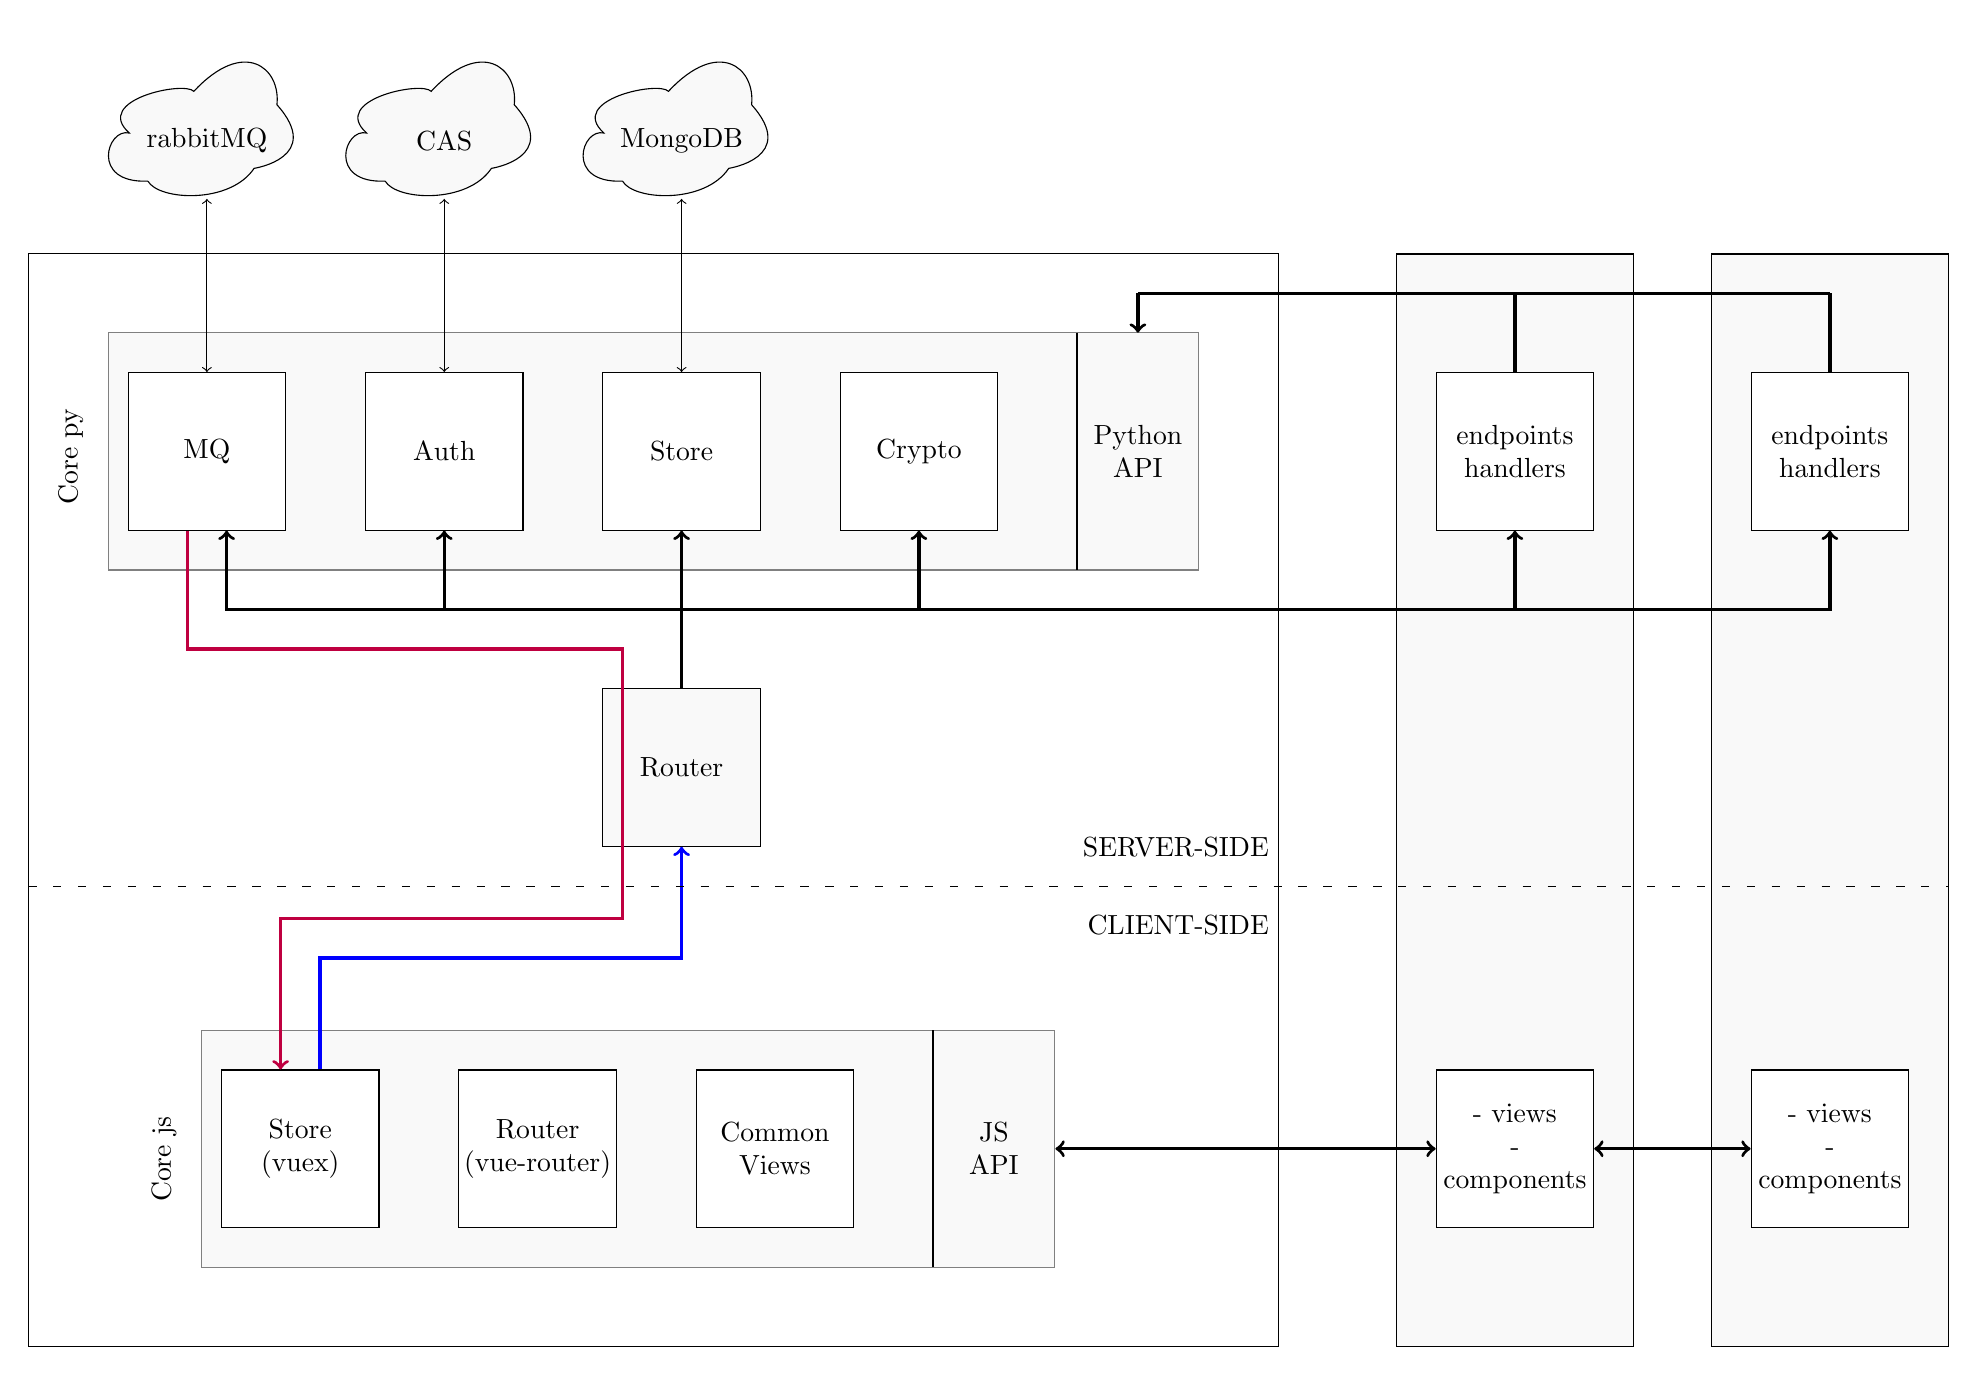
\begin{tikzpicture}
%core Python part
\node[rectangle, draw, minimum size=2cm, fill=white] (mq) {MQ};
\node[rectangle, draw, minimum size=2cm, right=of mq, fill=white] (auth) {Auth};
\node[rectangle, draw, minimum size=2cm, right=of auth, fill=white] (store) {Store};
\node[rectangle, draw, minimum size=2cm, right=of store, fill=white] (crypto) {Crypto};
\node[rectangle, left =  .cm of mq, minimum size=0cm] (for_space_Python){};
%wrapper for core Python objects
\node[rectangle,  minimum width=1cm, minimum height= 3cm, right=of crypto, text width=1.3cm, align=center] (Pythonapi) {Python\\API};
\draw (Pythonapi.north west) -- (Pythonapi.south west);
\begin{scope}[on background layer]
\node [draw=black!50, fit={(for_space_Python)(mq)(auth)(store)(crypto)(Pythonapi)}, inner sep=0, fill=gray!5] (core_Python) {};
 \end{scope}
%rotated label
\node[label={[label distance=-.8cm, text depth=-1ex,rotate=90, align=center]right:Core py}, align=center,  left=.5cm of core_Python] {};
%router object
\node[rectangle, draw, minimum size=2cm, below=2cm of store, fill=gray!5] (router) {Router};
%core js part
\node[rectangle, draw, minimum size=2cm, below left=4cm of router, text width=2cm, align=center, inner sep=0, fill=white] (js_store) {Store\\ (vuex)};
\node[rectangle, draw, minimum size=2cm, right=of js_store, text width=2cm, align=center, inner sep=0, fill=white] (js_router) {Router (vue-router)};
\node[rectangle, draw, minimum size=2cm, right=of js_router, text width=2cm, align=center, inner sep=0, fill=white] (com_views) {Common Views};
\node[rectangle, left =  .cm of js_store, minimum size=0cm] (for_space_js){};

%wrapper for core js objects
\node[rectangle,  minimum width=1cm, minimum height= 3cm, right=of com_views, text width=1.3cm, align=center] (jsapi) {JS\\API};
\draw (jsapi.north west) -- (jsapi.south west);
\begin{scope}[on background layer]
\node [draw=black!50, fit={(for_space_js) (js_store)(js_router)(com_views)(jsapi)}, inner sep=0, align=left, fill=gray!5] (core_js) {\hspace*{.5cm}};
 \end{scope}
%rotated label
\node[label={[label distance=-.8cm, text depth=-1ex,rotate=90, align=center]right:Core js}, align=center,  left=.5cm of core_js] {};
%big tozti wrapper
\node[rectangle, draw, fit={(core_js)(core_Python)}, inner sep=1cm] (tozti) {};
%extension A
\node[rectangle, draw, minimum size=2cm, right=3cm of core_Python, text width=2cm, align=center, inner sep=0, fill=white] (a_Python) {endpoints handlers};
\node[rectangle, draw, minimum size=2cm, text width=2cm, align=center, inner sep=0, fill=white] at (core_js -| a_Python) (a_js) {- views\\- components};
\begin{scope}[on background layer]
\node[rectangle, draw,fit={(a_js)(a_Python)}, inner sep=.5cm, inner ysep=1.5cm, fill=gray!5] (a_extension) {};
 \end{scope}
 %extension B
\node[rectangle, draw, minimum size=2cm, right=7cm of core_Python, text width=2cm, align=center, inner sep=0, fill=white] (b_Python) {endpoints handlers};
\node[rectangle, draw, minimum size=2cm, text width=2cm, align=center, inner sep=0, fill=white] at (core_js -| b_Python) (b_js) {- views\\- components};
\begin{scope}[on background layer]
\node[rectangle, draw,fit={(b_js)(b_Python)}, inner sep=.5cm, inner ysep=1.5cm, fill=gray!5] (b_extension) {};
 \end{scope}
% links everywhere
\draw[->, very thick] (router.north) to[|-|] ([xshift=.25cm]mq.south);
\draw[->, very thick] (router.north) to[|-|] (auth.south);
\draw[->, very thick] (router.north) to[|-|] (store.south);
\draw[->, very thick] (router.north) to[|-|] (crypto.south);
\draw[->, very thick] (router.north) to[|-|] (a_Python.south);
\draw[->, very thick] (router.north) to[|-|] (b_Python.south);
\draw[->, very thick, blue] ([xshift=.25cm]js_store.north) to[|-|] (router.south);
\draw[->, very thick, purple] ([xshift=-.75cm]router.center)  to[|-|] ([xshift=-.25cm]js_store.north) ;
\draw[-, very thick, purple] ([xshift=-.75cm]router.center)  to[|-|] ([xshift=-.25cm]mq.south) ;
\draw[<->, very thick](b_js) -- (a_js);
\draw[<->, very thick](core_js) -- (a_js);
\draw[->, very thick]([yshift=.5cm]Pythonapi.north) -- (Pythonapi.north);
\draw[-, very thick]([yshift=.5cm]Pythonapi.north -| a_Python.north) -- (a_Python.north);
\draw[-, very thick]([yshift=.5cm]Pythonapi.north -| b_Python.north) -- (b_Python.north);
\draw[-, very thick]([yshift=.5cm]Pythonapi.north -| b_Python.north) -- ([yshift=.5cm]Pythonapi.north);
%three clouds
 \node[above= 2cm of mq] (cloud_mq) {\tikz \asymcloud[.11]{fill=gray!5};};
 \node[align=center] at([yshift=-.25cm]cloud_mq) {rabbitMQ};
\draw[<->]([yshift=.2cm]cloud_mq.south) -- (mq);
 \node[above= 2cm of auth] (cloud_auth) {\tikz \asymcloud[.11]{fill=gray!5};};
 \node[align=center] at([yshift=-.25cm]cloud_auth) {CAS};
\draw[<->]([yshift=.2cm]cloud_auth.south) -- (auth);
 \node[above= 2cm of store] (cloud_store) {\tikz \asymcloud[.11]{fill=gray!5};};
 \node[align=center] at([yshift=-.25cm]cloud_store) {MongoDB};
\draw[<->]([yshift=.2cm]cloud_store.south) -- (store);
% separator server-side / client side
\draw[-, loosely dashed] ([yshift=-.5cm]router.south -| tozti.west) -- ([yshift=-.5cm]router.south -| b_extension.east);
\node[align=right, anchor=east] at (router.south -| tozti.east) {SERVER-SIDE};
\node[align=right, anchor=east] at ([yshift=-1cm]router.south -| tozti.east) {CLIENT-SIDE};
\end{tikzpicture}
\end{turn}
    \caption{Architecture diagram}
    \label{fig:architecture schema}
\end{figure}
\restoregeometry

\subsection{Backend}
% back-end:
%   * Python with asyncio, maybe pypy at some point
%   * http server: aiohttp, simple stupid
%   * storage:
%     * mongodb backend
%     * jsonapi

The backend consists of three communicating components: the core HTTP server, the MongoDB storage server and the RabbitMQ message broker. The purpose of the core server is to act as a middleman between the frontend and the storage server. It validates the incoming data, renders the outgoing data, and takes care of the permissions for accessing data in the storage. It is written in Python, and uses the \texttt{asyncio} library for scheduling asynchronous IO operations such as database accesses and HTTP requests. The communication with the frontend is done through a HTTP API, that is heavily inspired by JSON API\cite{jsonapi}. Extensions can introduce new functionality by installing new HTTP endpoint handlers in the core HTTP server.

\subsection{HTTP API}
\subsubsection{JSON API}
A JSON API inspired API has been chosen because it follows the well-known \emph{HATEOS} architecture (Hypertext As The Engine Of Application State). This essentially means that the client need not to construct URLs \emph{ex nihilo} to navigate the API: a single entry point is needed, after which URLs for all related actions will be provided inside the HTTP reply. This means that the state of the client \emph{is} the document in the reply, and possible state transitions are all included as hyperlinks inside this state. The benefit of HATEOAS---in addition to being the 3\textsuperscript{rd} and highest level of RESTful API design---is that it makes the API more discoverable and clients more robust. Such a strong contract between the client and the servers enables us to keep the client unmodified, even in face of relatively large changes, such as server hostname change, URL change or type description change (see below).

JSON API is centered around \emph{resource objects}. They are what we would call \emph{entities} in databases or \emph{hypermedia} on the web. A resource object is a simple abstract structure: it has an unique ID, a type, some arbitrary attributes, meta-data and finally some \emph{relationships}.

A relationship is a named link between the current resource and either one or many target resources. This enables us to create a directed tagged graph between resources and build complex data-structures like a file system or an identity management system.

\subsubsection{Type Description Objects}
Types are not defined in the JSON API specification, they are just treated as opaque identifiers. We decided to use an URL to a JSON file as type identifiers. This JSON file must contain a \emph{type description object}. This type description lists the allowed (and required) attributes, together with a JSON-Schema\cite{jsonschema} specifying what are the allowed values for each attribute. It also contains a description of the relationships for that type, that is for each relation name, whether it is \emph{to-one} or \emph{to-many} and what types the targets can have.

For example, the \texttt{/types/group.json} type might specify a \emph{to-many} relationship called \texttt{members}, whose targets are restricted to the \texttt{/types/user.json} type.

This creates a directed graph, but regularly we want to have bidirectional links where both directions are kept in sync. For example, we would like \texttt{/types/user.json} to specify a relationship named \texttt{groups} mapping to the list of \texttt{/types/group.json} it is a member of. To handle that, we add a new kind of relationship description: \emph{reverse-of} relationships. These relationships cannot be modified by the user, they are specified by a target type and a forward-relationship name---here \texttt{/types/group.json} and \texttt{members}. This relationship is not kept in the internal database, but upon query of a given object we fill it we the result of the query ``all resources of matching type such that the current resource is contained in the matching relationship''.

\subsubsection{Authentication}
To perform a login, we will use state-of-the-art Argon2 password hashing from the libsodium\cite{libsodium} library. We might do the actual hashing on the client-side, for efficiency. We might also implement additional login schema like CAS (to integrate with the ENS de Lyon single sign-on), GPG authentication (for power-users that have a key), TOTP\cite{rfc6238} or U2F\cite{U2F} (for power-users that have a hardware security token).

Upon login, the server will issue a cookie that the user will include in each of it's next requests to authenticate itself. We have surveyed several systems to do this and the possibilities boiled down to: JSON Web Tokens\cite{jwt}, Macaroons\cite{macaroons} or rolling our own simple scheme using a public-key signatures. We eliminated JSON Web Tokens because of bad comments\cite{jwthn} and because they provide little advantage over rolling our own solution. We did not decide yet, but we might prefer Macaroons since it is an already-specified system and because it provides advanced functionality like delegation and caveats.

\subsubsection{Endpoints}
Our API provides all specified endpoints to operate on resources and resources. For more information on our divergences from the JSON API specification, see \url{https://github.com/tozti/tozti/pull/4}. Summary of the API endpoints:

\begin{description}
  \item[\texttt{POST /api/store/resources},] create a new resource object
  \item[\texttt{ANY /api/store/resources/\{id\}},] get, patch, put or delete a specific resource object
  \item[\texttt{ANY /api/store/resources/\{id\}/\{rel\}},] get, append or replace a specific relationship object
  \item[\texttt{GET /api/store/me},] an alias to get the \texttt{/types/user.json} resource object of the authentificated user doing the request
  \item[\texttt{POST /api/store/upload},] upload binary data such as media files and return a permalink to it
  \item[\texttt{POST /api/auth/login},] perform a login
  \item[\texttt{WebSocket /api/mq/\{channel\}},] listen to messages on a specific channel
\end{description}

\subsection{Frontend}

The frontend follows the ``single-page application'' approach, which is the \emph{de facto} standard for modern web application development. Essentially, it means that the application interacts with the user by rewriting the current page rather than loading new pages from the server, which improves the user experience by making the whole application feel more responsive. 

In this approach, the client retrieves most of the application logic on the first request to the website. This includes the routing layer (which tells the browser which page to render depending on the URL) and the rendering layer (which describes the HTML code to produce for a given type of resource). This way, subsequent page changes do not trigger a full page refresh: instead, the client uses the HTTP API to retrieve JSON objects for the resources that need to be displayed, and renders them locally.

Specifically, our implementation uses well-established tools such as Vue\cite{vuejs}, Vuex\cite{vuex} and Vue Router\cite{vuerouter} to help with the routing, state management and rendering. Like most recent web frameworks, Vue allows for declarative rendering of small, reusable components, which simplifies the development of single-page applications. This way, even developers with limited web development skills can write relatively robust and modular code. Working with small components also allows us to easily \textbf{create new views and extend existing ones}, as required by chapter \ref{chap:Specification}.

% front-end:
% single page app
% uses declarative programming
% separated into components
% uses vuejs/vuex
% 
%   * coded with vuejs & vuex (reactive programing)
%   * explain how components are great (to export them, extend, polymorphic components...)
%   * 

\section{User Experience}
In order to streamline the development process, we created mockups for the most complex components, so that their design is already known at implementation time. This process is known to save (developer) time, as it allows them to focus on actual code, as opposed to design and usability concerns. The mockups can be found in chapter \ref{chap:mockups}.

\subsection{Taxonomy}
As specified, we want a consistent organisation of the resources (a taxonomy). Usually, this is done with a resource hierarchy, that is a tree. However, a common requirement is to share some resource with multiple people. On a file system this is usually done with symbolic links. Our approach for the taxonomy is closer to hard links than symbolic links: we allow resources to show up at multiple places in the tree. This taxonomy could also be described as being the crossover of a tag system and a tree: the set of tags form a tree and every resource can be tagged one or more times.

\subsection{Common Ground}
There are two UI elements that we want to be present in every view of \tozti. First a thin horizontal header at the top containing the profile, settings and notification menu. Second a vertical strip on the left containing quick-links to some root points in the tree. This quick-links will contain the root directory of every group the user is a member of but will also be customisable by the users. See the top left drawing of figure \ref{fig:mockup-calendar} for these common parts.

\subsection{Core Views}
Besides the user profile, group profile and settings views that we did not describe yet, there are two views that are provided by the core.

The first one is the \emph{directory} view, that is the consistent view of directory (also called tag) of the taxonomy. As such it can be compared to the main window of a file browser or to \emph{categories list} view in bulletin-boards. The content of the view is straightforward: the main pane will be filled by a vertical list of lines, each describing an element of the directory. Each line will show the name of that element and some additional information based on it's type (it can be a file, a thread, an event or a subdirectory). To We might add a full-height column on the right of the pane showing a small preview, meta-data and interactions like \emph{share-to} or \emph{edit} when the user selects a line. See figure \ref{fig:mockup-taxo}.

The second one is the dashboard and landing page. This view is much more versatile and can be extended at will with new widgets. We haven't yet fully specified how it should look like, but most likely it will be a set of rectangular tiles (one or two columns), showing things like \emph{upcoming events}, \emph{recently modified resources} etc.

\subsection{File}
The (media) file extension will provide the full-page view of a given file. This view will contain a meta-data column on the right like the \emph{directory} view. The rest of the pane will be occupied with the file viewer itself (a media player, image viewer or PDF viewer). We might add a history of actions (to whom it was shared, when did who change it, etc.) below the viewer.

\subsection{Calendar}
The \emph{calendar} extension is centered around \emph{events}. Events will be presented in the form of a calendar (grid where columns and rows corresponds to a specific day and time). Events can be shared between groups of persons or restricted to a sub-group of the current group. This notion of sharing and restricting is integrated directly thanks to the \textit{taxonomy}. Furthermore, events can be defined to be periodic or punctual. As such, the calendar view is made of two big components:
\begin{itemize}
\item A search bar with some controls to search through specific events, see the events planned later or earlier in time, and add an event.
\item A calendar displaying the events of the week, month and day
\end{itemize}
When a user double click on an event inside the calendar, an overlay page will allow him to view a more precise description of this event. He will be able, if he has the permissions to, to edit and delete this event. 
See figure \ref{fig:mockup-calendar} for more.

\subsection{Discussion}
The main resource type of the \emph{discussion} extension is the \emph{thread}. As such, it will provide a classical bulletin-board view of a given thread: a vertical sequence of messages followed by a message redaction zone. On the right we will add a full-height column displaying the list of resources that have been mentioned in the thread. For example the organisational thread of some upcoming event might mention resources like the public event, the staff task-attribution form or advertisement PDFs and images. See figure \ref{fig:mockup-discussion1} and \ref{fig:mockup-discussion2}.


\afterpage{\clearpage}
\newpage

\section{Cryptography}

\subsection{A bit of background}

First of all, here are some very rough descriptions of a few cryptographic terms we use.
\begin{itemize}
\item \emph{Homomorphic encryption:} A method of encrypting data, where the encoder commutes with some mathematical operations. In other words, a user can ask a third party (here, the server) to perform some operation $f$ on the encrypted data $e(D)$. The user can then retrieve $f(e(D))=e(f(D))$ and decrypt it in order to get $f(D)$. The third party gained no information about the encrypted data even though he was the one to perform the operation: with homomorphic encryption, one can edit data without having knowledge of it.
\item \emph{Asymmetric/public-key encryption:} A method where we use a pair of public-private keys. Once encrypted using the public key, a message can only be \emph{efficiently} decrypted using the matching private key.
\item \emph{Keychain:} Each user stores some of their keys on the server (in particular their public keys, but never their private keys).
\end{itemize}

\subsection{Our problem}
\subsubsection{Goals \& Motivations}
% Explain why we need crypto (cf testimonies, private data)
% Explain why we don't want the owner of the server to have access to the secrets (cf multiple servers)
When we surveyed prospective users of \tozti (i.e student associations), one particular use-case came up which requires us to set up cryptographic security: some associations have to collect very sensitive data such as testimonies of sexual harassment.

One important requirement for our storage system is that the server's owner cannot have access to the data. This is both for obvious privacy reasons, as well as to keep our hands free for if we want to distribute the data over multiple servers. Indeed, one long term project for the storage is to be compatible with multiple servers (an object of a certain type could for instance be stored on a server even though its type is only defined on another server). In that scenario, we cannot possibly trust an increasing number of server owners, even if we were ready to trust one.

For this very same reason, we require that all decryption to happen client-side. One possible way around this would be to use (fully) homomorphic encryption (FHE). Indeed that would allow some operations/modifications on encrypted data to be done server-side without allowing the owner of the server to gain access to any information.

\subsubsection{Choices \& Compromises}
% Vulnerable to side channel attack, no homomorphic encryption
While we cannot guarantee full anonymity for users storing their testimonies (an attacker listening in might be able to see that a user sent data) as not authenticating users would leave us wide open to Denial of Service (DDOS) attacks, we must guarantee the integrity and confidentiality of these testimonies.

Considering \tozti's use-case, (F)HE seems too complicated, and more importantly it would slow down every storage access. We therefore decided to forgo it entirely.

The cryptographic protocol we present here might be vulnerable to side channel attacks (depending on the libraries we use), but then again, considering the most general use-case (i.e everything but sensitive testimonies), it does not seem to matter at first (\tozti is not meant, \emph{as of yet}, to be used to store data so sensitive as to catch the eye of so resourceful an attacker). Still, before we launch \tozti we will have to do a proper security audit, analysing possible side-channels and implementation issues.

\subsection{Protocols}

\subsubsection{A general scheme}

\begin{notation}[Shorthand \& Notations]
\begin{itemize}
\item $pub_A$, $priv_A$ are Alice's public and private keys (for an asymmetric encryption algorithm).
\item Given a message $M$ and a key $\chi$, define $e_\chi(M)$ the encryption of $M$ using $\chi$ (this is a general notation, common to all encryption methods).
\end{itemize}
\end{notation}

\paragraph{Creating secret data}
% Alice wants to share her secret data
\emph{Case:} User Alice wants to store a message $M$ on the server.
\begin{itemize}
\item Alice generates (client-side) a key $K$ in order to encrypt $M$ (client-side).
\item Alice sends $e_K(M)$ to the server.
\item Alice encrypts (client-side) $K$ with $pub_A$.
\item Alice sends $e_{pub_A}(K)$ to her keychain on the server.
\end{itemize}

Notice that since the server does not have access to $priv_A$, it cannot efficiently compute $K$ and hence $M$.

\begin{figure}[!h]
\centering
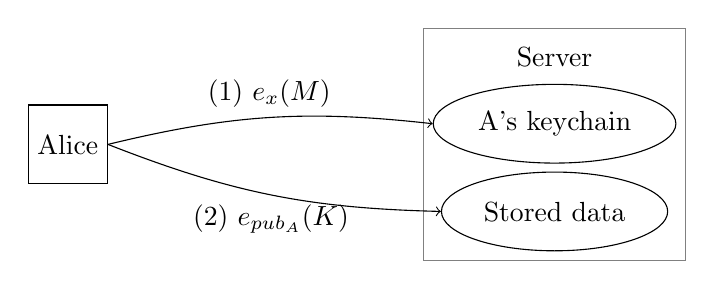
\begin{tikzpicture}
  \node (server_title) { Server };
\node[ellipse, draw=black, minimum height=1cm, below=.1cm of server_title] (a_keys) {A's keychain};
\node[ellipse, draw=black, minimum height=1cm, below=.1cm of a_keys.south] (stored_data) {Stored data};
  \node [draw=black!50, fit={(server_title) (a_keys) (stored_data)}] (server) {};
\node[rectangle, draw=black, minimum size=1cm, left=4cm of server] (Alice) {Alice};
\path[->]
	(Alice.east) edge [bend left=10] node[above] {(1) $e_x(M)$} (a_keys.west)
	(Alice.east) edge [bend right=10] node[below] {(2) $e_{pub_A}(K)$} (stored_data.west)
;		
\end{tikzpicture}
\label{creating_secret_data}
\caption{Creating secret data}
\end{figure}

\paragraph{Retrieving secret data}

\emph{Case:} User Alice wants to retrieve the message $M$ which is stored on the server.
\begin{itemize}
\item Alice sends the request to the server.
\item The server checks if she is allowed access (via a tag attached to the secret message).
\item If she is, the server sends Alice $e_K(M)$ and $e_{{pub}_A}(K)$ (the latter retrieved from Alice's keychain).
\item Alice decrypts (client-side) $e_{{pub}_A}(K)$ using ${priv}_A$ in order to obtain $K$~.
\item Alice decrypts (client-side) $e_{K}(M)$ using $K$ in order to obtain $M$~.
\end{itemize}

\begin{figure}[!h]
\centering
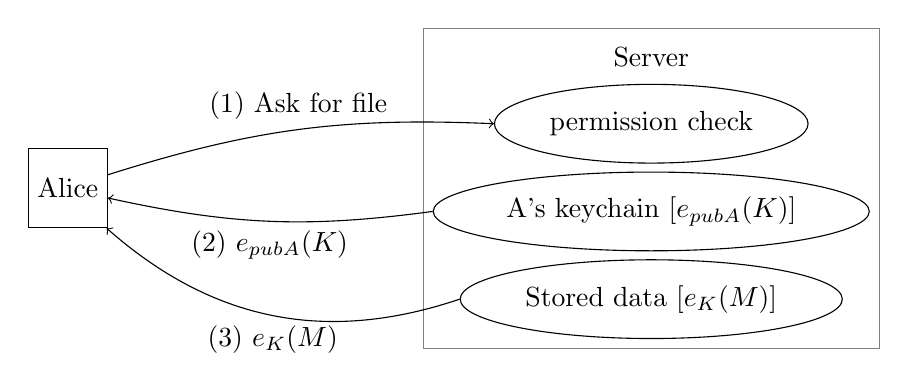
\begin{tikzpicture}
  \node (server_title) { Server };
\node[ellipse, draw=black, minimum height=1cm, below=.1cm of server_title] (permissions) {permission check};
\node[ellipse, draw=black, minimum height=1cm, below=.1cm of permissions] (a_keys) {A's keychain $[e_{pubA}(K)]$};
\node[ellipse, draw=black, minimum height=1cm, below=.1cm of a_keys.south] (stored_data) {Stored data $[e_K(M)]$};
  \node [draw=black!50, fit={(server_title) (permissions) (a_keys) (stored_data)}] (server) {};
\node[rectangle, draw=black, minimum size=1cm, left=4cm of server] (Alice) {Alice};
\path[->]
	(Alice) edge [bend left=10] node[above] {(1) Ask for file} (permissions.west)
	(a_keys.west) edge [bend left=10] node[below] {(2) $e_{pubA}(K)$} (Alice) 
	(stored_data.west) edge [bend left=30] node[below] {(3) $e_ {K}(M)$} (Alice) 
;		
\end{tikzpicture}
\label{retrieving_secret_data}
\caption{Retrieving secret data}
\end{figure}

\paragraph{Sharing secret data}

\emph{Case:} User Alice wants to share with user Bob the message $M$ which is stored as $e_{{pub}_A}(M)$ on the server.
\begin{itemize}
\item Alice retrieves $pub_B$ from B's keychain on the server.
\item Alice retrieves $e_{{pub}_A}(K)$ from her keychain on the server.
\item Alice decrypts (client-side) $e_{{pub}_A}(K)$ to get $K$ and encrypts it (client-side) using $pub_B$~.
\item Alice sends $e_{pub_B}(K)$ to Bob's keychain.
\item Bob now has access to $K$, hence $M$~.
\end{itemize}

\begin{figure}[!h]
\centering
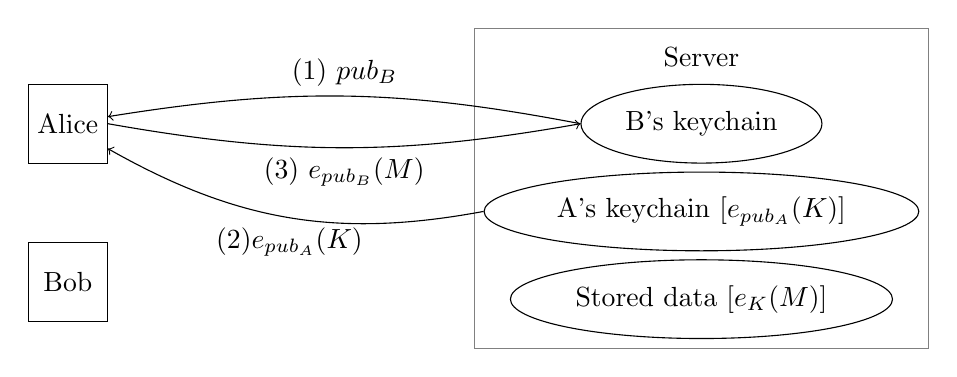
\begin{tikzpicture}
  \node (server_title) { Server };
\node[ellipse, draw=black, minimum height=1cm, below=.1cm of server_title] (b_keys) {B's keychain };
\node[ellipse, draw=black, minimum height=1cm, below=.1cm of b_keys] (a_keys) {A's keychain $[e_{pub_A}(K)]$};
\node[ellipse, draw=black, minimum height=1cm, below=.1cm of a_keys] (stored_data) {Stored data $[e_K(M)]$};
  \node [draw=black!50, fit={(server_title) (b_keys) (a_keys) (stored_data)}] (server) {};
\node[rectangle, draw=black, minimum size=1cm, left=6cm of b_keys] (Alice) {Alice};
\node[rectangle, draw=black, minimum size=1cm, left=4cm of server, below=of Alice] (Bob) {Bob};
\path[->]
	(a_keys.west) edge [bend left=20] node[below] {(2)$e_{pub_A}(K)$ } (Alice) 
	(b_keys.west) edge [bend right=10] node[above] {(1) $pub_B$} (Alice) 
	(Alice.east) edge [bend right=10] node[below] {(3) $e_ {pub_B}(M)$} (b_keys.west) 
;		
\end{tikzpicture}
\label{sharing_secret_data}
\caption{Sharing secret data}
\end{figure}

\paragraph{Group keys}
% TODO
This is a generalisation of sharing secret data amongst multiple users. Each group has a symmetric key (which all members share). In order to save memory space on the server, the group can also share a keychain, so as not to copy the group's keys in every one of the group's members keychains.

This approach has two major deficiencies however:
\begin{itemize}
\item \emph{Confidentiality:} The group's confidentiality is only as strong as its weakest link, and it is unreasonable to assume that all members of a large group have good security practices.
\item \emph{Computation time:} Whenever a member leaves a group, all of the group's keys have to be generated anew. This is computationally long, especially for larger groups of users. Once the system is implemented, and depending on the efficiency of our key generation algorithms, we might have to think of a better way to share a secret amongst a group.
\end{itemize}
Still, this is the best compromise we have between security and ergonomy.

\subsubsection{Implementation recommendations}
\paragraph{Possible encryption schemes}
% The various (a)symmetric primitives
  Our high-level protocol relies on us having some means of performing both asymmetric and symmetric encryption. Here are the algorithms which we plan on using:
\begin{itemize}
\item for asymmetric encryption: either Curve25519 (which offers 128 bits of security on elliptic curves, and is good with broken random number generators), or RSA (at least with 2048 bit keys, since under 1024 bits is broken).
\item for symmetric encryption: Advanced Encryption Standard (AES) or ChaCha20-Poly1305 (modern and has authentication).
\end{itemize}
\paragraph{Libraries}
For the moment, the library we plan on using is the JavaScript version of \texttt{libsodium}.

\chapter{Status Report}
Our code is hosted in on GitHub at \url{github.com/tozti}. We separated the repositories for the core (\texttt{tozti.git}) and the extensions (\texttt{tozti-calendar.git}, \texttt{tozti-discussion.git}, \dots). Our website is at \url{tozti.github.io} and the documentation can be found at \url{tozti.readthedocs.io}.

\section{Current State}
Our most important achievement up to now is probably that we have finalised the precise specification of the backend and the frontend. This was a complicated task because of the multiple components in the code and the need for modularity, something that is not that common for such webapps. As such, we have taken particular care to think about a lot of practical implementation problems we would encounter in some architecture or another.

Broken down according to the individual workpackages, the current status can be summarised as follows:
\begin{description}
	\item[Architecture] Defined the architecture of the entire system. This also included writing all the \emph{infrastructure} code, that is the helpers to make extensions possible on the client and on the server.
    \item[Calendar] Created mockups and defined a precise specification to answer to the user requests. Also wrote user stories to support our specification.
    \item[Com] Met with potential users of \tozti and asked them what their needs are. Filled the website.
    \item[Media] Created mockups and some rough start of the Vue code.
    \item[Discussion] Created mockups of the bulletin-board and defined a precise specification to answer to the user requests. Also wrote user stories to support our specification.
    \item[Meta] Built \tozti's website. Wrote tutorials and documentation around the core on how to create extensions.
    \item[Storage] Implemented most of the JSON API endpoints of the store, together with interface to the MongoDB backend. Designed the cryptographic scheme.
    \item[UX] Designed the global UX of the website: the dashboard vs taxonomy view and the areas that will be present in every page of the app.
\end{description}

\section{Next Steps}
Now that the specification is more or less stable, the idea is to continue polishing the core, as well as to develop the extensions beyond the initial mockup stage. 
On the client-side, this includes:
\begin{itemize}
  \item Implementing the local resource store and API client around Vuex.
  \item Documenting the API more extensively instead of offloading to the JSON API specification.
  \item Implementing cryptographic computations.
  \item Continuing the working existing, and implementing new extensions.
  \item Factoring out the most common UI components used by different extensions into the core.
  \item Unifying the design language of all extensions (writing a common UI kit).
\end{itemize}
On the server-side, this includes:
\begin{itemize}
  \item Completing the storage API, and bringing it in line with the specification.
  \item (Designing and) implementing the authentication layer on top of the API.
  \item Implementing the message queue, for sending notifications to the client.
  \item Implementing the encryption layer on top of the storage API. The cryptographic computations themselves are going to be done on the client, but the storage layer need to be made aware of that fact.
\end{itemize}

Finally, common to both parts is the necessity to implement the continuous integration and test infrastructure, that will allow as to detect regressions early, and avoid committing faulty code to the repository. Additionally, as the codebase evolves, it will be the duty of the teams to document both the inner workings and the public interface of their code. This will make it easier for future external collaborators to extend to \tozti core and implement new extensions.
% think to put there
% Think about the CSSRF stuff. We said it does not matter, but we are also saying some associations wants to store secured data. So ?
% Do tests
% Polish the core
% More docs & more docs
% Do extensions until death

\appendix
\label{chap:mockups}
\chapter{Mockups}

\begin{figure}[h]
\centering
\includegraphics[width=\linewidth,trim={0 1cm 0 0},clip]{mockups/directory.jpg}
\caption{A mockup of the directory view.}
\label{fig:mockup-taxo}
\end{figure}

\begin{figure}[h]
\centering
\includegraphics[width=\linewidth,trim={0 1cm 0 1cm},clip]{mockups/calendar-flupe.png}
\caption{Mockup of the calendar}
\label{fig:mockup-calendar}
\end{figure}

\begin{figure}[h]
\centering
\includegraphics[width=\linewidth,trim={0 1cm 0 1cm},clip]{mockups/discussion-alex.pdf}
\caption{A mockup of the forum}
\label{fig:mockup-discussion1}
\end{figure}

\begin{figure}[h]
\centering
\includegraphics[width=\linewidth,trim={0 1cm 0 1cm},clip]{mockups/discussion-flupe.png}
\caption{Another mockup of the forum}
\label{fig:mockup-discussion2}
\end{figure}


\printbibliography

\end{document}
